\documentclass[12pt,a4paper]{article}

\usepackage{amsmath}
\usepackage{amssymb}
\usepackage{graphicx}
\usepackage{CJKutf8}

\graphicspath{images/} %TODO

\title{Homework 1} %TODO
\author{Qijun Han 12212635}
\date{\today}


\begin{document}
\maketitle

\section{NE1.1}
\subsection*{Problem a}

\[G(s) = \frac{1}{s^2+2s+6}\]

ODE:
\[y''(t) + 2y'(t) + 6y(t) = u(t)\]

let $x_1(t) = y(t), x_2(t) = y'(t)$, then we have

$\begin{cases}
    x_1'(t) = x_2(t) \\
    x_2'(t) = -2x_2(t) - 6x_1(t) + u(t)
\end{cases}
$

so the state space representation is
\begin{equation}
    \begin{aligned}
        \begin{bmatrix}
            {x_1(t)} \\
            {x_2(t)}
        \end{bmatrix}' & = \begin{bmatrix}
                               0  & 1  \\
                               -6 & -2
                           \end{bmatrix} \begin{bmatrix}
                                             x_1(t) \\
                                             x_2(t)
                                         \end{bmatrix} + \begin{bmatrix}
                                                             0 \\
                                                             1
                                                         \end{bmatrix} u(t) \\
        y(t)               & = \begin{bmatrix}
                                1 & 0
                            \end{bmatrix} \begin{bmatrix}
                                              x_1(t) \\
                                              x_2(t)
                                          \end{bmatrix}
    \end{aligned}
\end{equation}

thus
$
    \mathbf{A} =
    \begin{bmatrix}
        0  & 1  \\
        -6 & -2
    \end{bmatrix},
    \mathbf{B} =
    \begin{bmatrix}
        0 \\
        1
    \end{bmatrix},
    \mathbf{\mathbf{C}} = \begin{bmatrix}
        1 & 0
    \end{bmatrix},
    \mathbf{D} =
    \begin{bmatrix}
        0
    \end{bmatrix}
$

\subsection*{Problem b}
let $G_1(s)=\frac{1}{s^2+2s+6}=\frac{W(s)}{U(s)}$, $G_2(s)=s+3=\frac{Y(s)}{W(s)}$, then
\[G(s)  = G_1(s)G_2(s) \]
ODE:
\begin{equation}
    \begin{aligned}
        w''(t) + w'(t) + w(t) & = u(t)    \\
        y(t)            & = w'(t) + 3w(t)
    \end{aligned}
\end{equation}
let $ x_1(t) = w(t), x_2(t) = w'(t)$, then we have
\begin{equation}
    \begin{aligned}
        \begin{bmatrix}
            {x_1(t)} \\
            {x_2(t)}
        \end{bmatrix}' & = \begin{bmatrix}
                               0  & 1  \\
                               -6 & -2
                           \end{bmatrix} \begin{bmatrix}
                                             x_1 \\
                                             x_2
                                         \end{bmatrix} + \begin{bmatrix}
                                                             0 \\
                                                             1
                                                         \end{bmatrix} u(t)
    \end{aligned}
\end{equation}
and
\[ y(t) = \begin{bmatrix}
        3 & 1
    \end{bmatrix} \begin{bmatrix}
                      x_1(t) \\
                      x_2(t)
                  \end{bmatrix} \]

thus
$
    \mathbf{A} =
    \begin{bmatrix}
        0  & 1  \\
        -6 & -2
    \end{bmatrix},
    \mathbf{B} =
    \begin{bmatrix}
        0 \\
        1
    \end{bmatrix},
    \mathbf{\mathbf{C}} = \begin{bmatrix}
        3 & 1
    \end{bmatrix},
    \mathbf{D} =
    \begin{bmatrix}
        0
    \end{bmatrix}
$

\subsection*{Problem c}
similar to (a), we have
$
\mathbf{A} = \begin{bmatrix}
    0  & 1 & 0  \\
    0 & 0 & 1 \\
    -6 & -8 & -4
\end{bmatrix},
\mathbf{B} = \begin{bmatrix}
    0 \\
    0 \\
    10
\end{bmatrix},
\mathbf{\mathbf{C}} = \begin{bmatrix}
    1 & 0 &0
\end{bmatrix},
\mathbf{D} = \begin{bmatrix}
    0
\end{bmatrix}
$

\subsection*{Problem d}
similar to (b), we have
$
\mathbf{A} = \begin{bmatrix}
    0 & 1 & 0 & 0 \\
    0 & 0 & 1 & 0 \\
    0 & 0 & 0 & 1 \\
    -66 & -44 & -11 & -10 \\
\end{bmatrix},
\mathbf{B}= \begin{bmatrix}
    0 \\
    0 \\
    0 \\
    1
\end{bmatrix},
\mathbf{\mathbf{C}}= \begin{bmatrix}
    6 & 4 & 1 & 0
\end{bmatrix},
\mathbf{D} = \begin{bmatrix}
    0
\end{bmatrix}
$

\section{AE1.11}

suppose $\mathbf{A}$ is an $m \times m$ matrix, $\mathbf{B}$ is an $n \times n$ matrix.
to prove
\[
\begin{bmatrix}
    \mathbf{A} & \mathbf{D} \\
    \mathbf{\mathbf{C}} & \mathbf{B}
\end{bmatrix}^{-1} = \begin{bmatrix}
    \mathbf{A}^{-1}+\mathbf{E}\mathbf{\Delta}^{-1}\mathbf{F} & -\mathbf{E}\mathbf{\Delta}^{-1} \\
    -\mathbf{\Delta}^{-1}\mathbf{F} & \mathbf{\Delta}^{-1}
\end{bmatrix}
\], 
we need to prove that
\[
    \begin{bmatrix}
        \mathbf{A} & \mathbf{D} \\
        \mathbf{\mathbf{C}} & \mathbf{B}
    \end{bmatrix} \begin{bmatrix}
        \mathbf{A}^{-1}+\mathbf{E}\mathbf{\Delta}^{-1}\mathbf{F} & -\mathbf{E}\mathbf{\Delta}^{-1} \\
        -\mathbf{\Delta}^{-1}\mathbf{F} & \mathbf{\Delta}^{-1}
    \end{bmatrix} = \begin{bmatrix}
        I_m & \mathbf{0} \\
        \mathbf{0} & I_n
    \end{bmatrix}
\]

first, consider the left-top block:
\[
    \begin{aligned}
        \mathbf{A}(\mathbf{A}^{-1}+\mathbf{E}\mathbf{\Delta}^{-1}\mathbf{F}) + \mathbf{D}(-\mathbf{\Delta}^{-1}\mathbf{F}) & = \mathbf{AA^{-1}} + \mathbf{AE}\mathbf{\Delta}^{-1}\mathbf{F} - \mathbf{D}\mathbf{\Delta}^{-1}\mathbf{F} \\
                                                     & = \mathbf{I_m} + \mathbf{AE}\mathbf{\Delta}^{-1}\mathbf{F} - \mathbf{D}\mathbf{\Delta}^{-1}\mathbf{F}
    \end{aligned}
\]
since $\mathbf{E} = \mathbf{A}^{-1}\mathbf{D}$, we have $\mathbf{AE}\mathbf{\Delta}^{-1}\mathbf{F} = \mathbf{D}\mathbf{\Delta}^{-1}\mathbf{F}$, thus we get $\mathbf{I_m}$.

second, consider the right-top block:
\[
    \begin{aligned}
        \mathbf{A}(-\mathbf{E}\mathbf{\Delta}^{-1}) + \mathbf{D}(\mathbf{\Delta}^{-1}) & = -\mathbf{AE}\mathbf{\Delta}^{-1} + \mathbf{D}\mathbf{\Delta}^{-1} \\
                                          & = -\mathbf{D}\mathbf{\Delta}^{-1} + \mathbf{D}\mathbf{\Delta}^{-1} \\
                                          & = \mathbf{0}
    \end{aligned}
\]

third, consider the left-bottom block:
\[
    \begin{aligned}
        \mathbf{\mathbf{C}}(\mathbf{A}^{-1}+\mathbf{E}\mathbf{\Delta}^{-1}\mathbf{F}) + \mathbf{B}(-\mathbf{\Delta}^{-1}\mathbf{F}) 
        & = \mathbf{CA}^{-1} + \mathbf{CE}\mathbf{\Delta}^{-1}\mathbf{F} - \mathbf{B}\mathbf{\Delta}^{-1}\mathbf{F} \\
                                                & = \mathbf{CA}^{-1} + (\mathbf{CE} - \mathbf{B})\mathbf{\Delta}^{-1}\mathbf{F} \\
                                                & = \mathbf{CA}^{-1} + (\mathbf{B} - \mathbf{CA}^{-1}\mathbf{D})\mathbf{\Delta}^{-1}\mathbf{F} \\
                                                & = \mathbf{CA}^{-1} - \mathbf{\Delta} \mathbf{\Delta}^{-1} \mathbf{F} \\
                                                & = \mathbf{CA}^{-1} - \mathbf{F} \\
                                                & = \mathbf{0}
    \end{aligned}
\]
since $\mathbf{E} = \mathbf{A}^{-1}\mathbf{D}$, we have $\mathbf{CE}\mathbf{\Delta}^{-1}\mathbf{F} = \mathbf{B}\mathbf{\Delta}^{-1}\mathbf{F}$, thus we get $\mathbf{0}$.

fourth, consider the right-bottom block:
\[
    \begin{aligned}
        \mathbf{\mathbf{C}}(-\mathbf{E}\mathbf{\Delta}^{-1}) + \mathbf{B}(\mathbf{\Delta}^{-1}) & = -\mathbf{CA}^{-1}\mathbf{D}\mathbf{\Delta}^{-1} + \mathbf{B}\mathbf{\Delta}^{-1} \\
                                          & = (\mathbf{B} - \mathbf{CA}^{-1}\mathbf{D})\mathbf{\Delta}^{-1} \\
                                          & = \mathbf{\Delta}^{-1}\mathbf{\Delta} \\
                                          & = \mathbf{I_n}
    \end{aligned}
\]

thus we have proved that
\[
    \begin{bmatrix}
        \mathbf{A} & \mathbf{D} \\
        \mathbf{\mathbf{C}} & \mathbf{B}
    \end{bmatrix}^{-1} = \begin{bmatrix}
        \mathbf{A}^{-1}+\mathbf{E}\mathbf{\Delta}^{-1}\mathbf{F} & -\mathbf{E}\mathbf{\Delta}^{-1} \\
        -\mathbf{\Delta}^{-1}\mathbf{F} & \mathbf{\Delta}^{-1}
    \end{bmatrix}
\]
Q.E.D.

\section{AE1.12}
first, consider $\lambda \neq 0$ :

notice that the Jordan block is an upper triangular matrix, 
thus the inverse of a Jordan block is also an upper triangular matrix.

so we suppose the inverse of the k-th Jordan block has the form of:
\[
    \begin{bmatrix}
        a_{11} & a_{12} & \cdots & a_{1k} \\
        0      & a_{22} & \cdots & a_{2k} \\
        \vdots & \vdots & \ddots & \vdots \\
        0      & 0      & \cdots & a_{kk}

    \end{bmatrix}
\]
from the fact that the multiplication of a Jordan block and its inverse is an identity matrix, we have
\[
    \begin{bmatrix}
        \lambda & 1      & 0      & \cdots & 0      \\
        0       & \lambda & 1      & \cdots & 0      \\
        0       & 0      & \lambda & \cdots & 0      \\
        \vdots  & \vdots & \vdots & \ddots & \vdots \\
        0       & 0      & 0      & \cdots & \lambda
    \end{bmatrix} \begin{bmatrix}
        a_{11} & a_{12} & \cdots & a_{1k} \\
        0      & a_{22} & \cdots & a_{2k} \\
        \vdots & \vdots & \ddots & \vdots \\
        0      & 0      & \cdots & a_{kk}
    \end{bmatrix} = \begin{bmatrix}
        1 & 0 & \cdots & 0 \\
        0 & 1 & \cdots & 0 \\
        \vdots & \vdots & \ddots & \vdots \\
        0 & 0 & \cdots & 1
    \end{bmatrix}
\]
thus we have
\[
    \begin{aligned}
        a_{11} \lambda & = 1 \\
        a_{11} + \lambda a_{12} & = 0 \\
        a_{12} + \lambda a_{13} & = 0 \\
        \vdots & \\
        a_{22} \lambda & = 1 \\
        a_{22} + \lambda a_{23} &= 0 \\
        a_{23} + \lambda a_{24} &= 0 \\
        \vdots & \\
        a_{k-1 k-1} \lambda & = 1 \\
        a_{k-1 k-1} + \lambda a_{k-1 k} &= 0 \\
    \end{aligned}
\]

thus the inverse of the k-th Jordan block is
\[
    \begin{bmatrix}
        \frac{1}{\lambda} &- \frac{1}{\lambda^2} & \frac{1}{\lambda^3} & \cdots & (-1)^{k+1} \frac{1}{\lambda^{k}} \\
        0                 & \frac{1}{\lambda}     & -\frac{1}{\lambda^2} & \cdots & (-1)^{k} \frac{1}{\lambda^{k-1}} \\
        0                 & 0                     & \frac{1}{\lambda}     & \cdots & (-1)^{k+1} \frac{1}{\lambda^{k-2}} \\
        \vdots            & \vdots                & \vdots                & \ddots & \vdots \\
        0                 & 0                     & 0                     & \cdots & \frac{1}{\lambda}
    \end{bmatrix}
\]

if $\lambda = 0$, then the inverse does not exist.

\section{CME1.4}
the corresponding characteristic equation is
\[
\begin{aligned}
    w^{(4)}(t) + 6w^{(3)}(t) + 86w''(t) + 176w'(t) + 680w(t) = u(t) \\
    y(t) = 100w(t) + 20w'(t)+10w''(t)
\end{aligned}
\]

let$H_1(s)=\frac{W(s)}{U(s)}, H_2(s) = \frac{Y(s)}{W(s)}$,
then 
\[
    H_1(s) = \frac{1}{s^4+6s^3+86s^2+176s+680}
\]
\[ 
    H_2(s) = 10s^2+20s+100
\]
so the overal transfer function is
\[
    H(s) = H_1(s)H_2(2)= \frac{10s^2+20s+100}{s^4+6s^3+86s^2+176s+680}
\]

\section{CE1.1}
\subsection*{Problem a}
set the positive direction to be "right",
according to Newton's second law,
% \[ 
% u_1(t)+u_2(t)+u_3(t) = k_1 y_1(t)+k_4 y_3(t) 
% +c_1 y_1'(t)+c_4 y_3'(t)
% +m_1 y_1''(t)+m_2 y_2''(t)+m_3 y_3''(t)
% \]

\[
    \begin{aligned}
        u_1(t) &= k_1 y_1(t)+k_2(y_1(t)-y_2(t))
        +c_1 y_1'(t)+c_2(y_1'(t)-y_2'(t))
        +m_1 y_1''(t) \\
        u_2(t) &= k_2(y_2(t)-y_1(t))+k_3(y_2(t)-y_3(t))
        +c_2(y_2'(t)-y_1'(t))+c_3(y_2'(t)-y_3'(t))
        +m_2 y_2''(t) \\
        u_3(t) &= k_3(y_3(t)-y_2(t))+k_4 y_3(t)
        +c_3(y_3'(t)-y_2'(t))+c_4 y_3'(t)
        +m_3 y_3''(t) \\
    \end{aligned}
\]
the free-body diagram is shown in the figure below:
\begin{figure}[h]
    \centering
    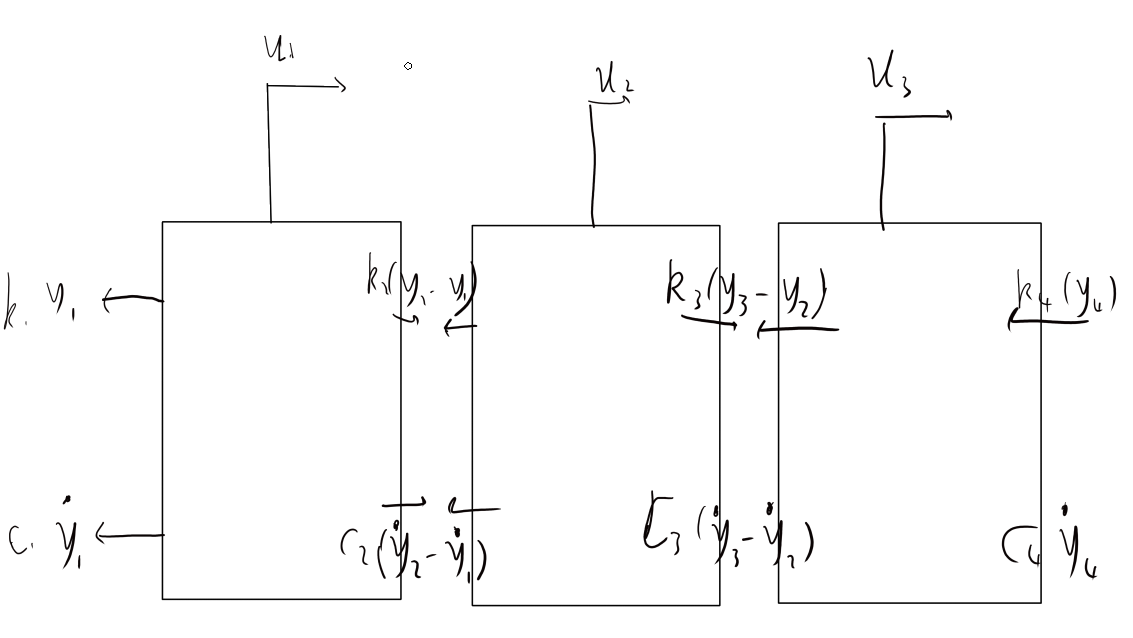
\includegraphics[width=0.8\textwidth]{assets/image.png}
    \caption{free-body diagram}
    \label{fig:free-body diagram}
\end{figure}


let 
$
    y(t) = 
    \begin{bmatrix}
        y_1(t) \\
        y_2(t) \\
        y_3(t)
    \end{bmatrix},
    u(t) =
    \begin{bmatrix}
        u_1(t) \\
        u_2(t) \\
        u_3(t)
    \end{bmatrix}
$, 
 the matrix-vector form is 
 \begin{equation}
    \begin{split}
    &\begin{bmatrix}
        m_1 & 0   & 0   \\
        0   & m_2 & 0   \\
        0   & 0   & m_3
    \end{bmatrix}
    \begin{bmatrix}
        y_1''(t) \\
        y_2''(t) \\
        y_3''(t)
    \end{bmatrix} + \\
    &\begin{bmatrix}
        c_1+c_2         & -c_2             & 0              \\
        -c_2            & c_2+c_3         & -c_3       \\
        0               & -c_3           & c_3+c_4
    \end{bmatrix}
    \begin{bmatrix}
        y_1'(t) \\
        y_2'(t) \\
        y_3'(t)
    \end{bmatrix} + \\
    &\begin{bmatrix}
        k_1+k_2         & -k_2             & 0              \\
        -k_2            & k_2+k_3         & -k_3       \\
        0               & -k_3           & k_3+k_4
    \end{bmatrix}
    \begin{bmatrix}
        y_1(t) \\
        y_2(t) \\
        y_3(t)
    \end{bmatrix} = \\
    &\begin{bmatrix}
        u_1(t) \\
        u_2(t) \\
        u_3(t)
    \end{bmatrix}
    \end{split}
\end{equation}

thus 
$\mathbf{M} = \begin{bmatrix}
    m_1 & 0   & 0   \\
    0   & m_2 & 0   \\
    0   & 0   & m_3
\end{bmatrix},
\mathbf{\mathbf{C}} = \begin{bmatrix}
    c_1+c_2         & -c_2             & 0              \\
    -c_2            & c_2+c_3         & -c_3       \\
    0               & -c_3           & c_3+c_4
\end{bmatrix}$
and

$
\mathbf{K} = \begin{bmatrix}
    k_1+k_2         & -k_2             & 0              \\
    -k_2            & k_2+k_3         & -k_3       \\
    0               & -k_3           & k_3+k_4
\end{bmatrix}
$

\subsection*{Problem b}
let
\[
    \begin{aligned}
        x_1(t) &= y_1(t) \\
        x_2(t) &= y_2(t) \\
        x_3(t) &= y_3(t) \\
        x_4(t) &= y_1'(t) \\
        x_5(t) &= y_2'(t) \\
        x_6(t) &= y_3'(t)
    \end{aligned}
\]
\subsection*{i}

$\mathbf{u(t)} = \begin{bmatrix}
    u_1(t)\\
    u_2(t) \\
    u_3(t)
\end{bmatrix}
$, $\mathbf{y(t)} = \begin{bmatrix}
    y_1(t)\\
    y_2(t)\\
    y_3(t)
\end{bmatrix}
$, $\mathbf{x(t)} = \begin{bmatrix}
    x_1(t)\\
    x_2(t)\\
    x_3(t)\\
    x_4(t)\\
    x_5(t)\\
    x_6(t)
\end{bmatrix}
$
, so the state-space realization is

\[
    \mathbf{x'(t)} = \begin{bmatrix}
        \mathbf{0} & \mathbf{I}\\
        \mathbf{-\mathbf{M}^{-1}\mathbf{K}} & \mathbf{-\mathbf{M}^{-1}\mathbf{\mathbf{C}}}
    \end{bmatrix}
    \mathbf{x(t)}+ \begin{bmatrix}
        \mathbf{0}\\
        \mathbf{I}
    \end{bmatrix}\mathbf{u(t)}
\], and
\[
    \mathbf{y(t)} = \begin{bmatrix}
        \mathbf{I} & \mathbf{0}
    \end{bmatrix}
    \mathbf{x(t)} + 
        \mathbf{0}\mathbf{u(t)}
\]

thus, $\mathbf{A} = \begin{bmatrix}
    \mathbf{0} & \mathbf{I}\\
    \mathbf{-\mathbf{M}^{-1}\mathbf{K}} & \mathbf{-\mathbf{M}^{-1}\mathbf{\mathbf{C}}}
\end{bmatrix}$, $\mathbf{B} = \begin{bmatrix}
    \mathbf{0}\\
    \mathbf{I}
\end{bmatrix}$, $\mathbf{\mathbf{C}}=\begin{bmatrix}
    \mathbf{I} & \mathbf{0}
\end{bmatrix}$, $\mathbf{D}=\mathbf{0}$

\subsection*{ii}
we only care $u_1(t)$ and $u_3(t)$, that is to say, we apply a linear transformation
$L: R^2 \to R^3$ which takes $\begin{bmatrix}
    u_1(t)\\
    u_3(t)
\end{bmatrix} $ as input and outputs
$ \begin{bmatrix}
    u_1(t)\\
    0 \\
    u_3(t)
\end{bmatrix}
$, with $\mathbf{y(t)} = \begin{bmatrix}
    y_1(t)\\
    y_2(t)\\
    y_3(t)
\end{bmatrix}$
, the state-space realization is
\[
    \mathbf{x'(t)} = \begin{bmatrix}
        \mathbf{0} & \mathbf{I}\\
        \mathbf{-\mathbf{M}^{-1}\mathbf{K}} & \mathbf{-\mathbf{M}^{-1}\mathbf{\mathbf{C}}}
    \end{bmatrix}
    \mathbf{x(t)}+ \begin{bmatrix}
        \mathbf{0}\\
        \mathbf{I}
    \end{bmatrix}
    \begin{bmatrix}
        1 & 0 \\
        0 & 0 \\
        0 & 1
    \end{bmatrix}\mathbf{u(t)}
\]
, and
\[
    \mathbf{y(t)} = \begin{bmatrix}
        \mathbf{I} & \mathbf{0}
    \end{bmatrix}
    \mathbf{x(t)} + 
        \mathbf{0}\mathbf{u(t)}
\]
thus $\mathbf{A} = \begin{bmatrix}
    \mathbf{0} & \mathbf{I}\\
    \mathbf{-\mathbf{M}^{-1}\mathbf{K}} & \mathbf{-\mathbf{M}^{-1}\mathbf{\mathbf{C}}}
\end{bmatrix}
$, $ \mathbf{B} = \begin{bmatrix}
    0 & 0 \\
    0 & 0 \\
    1 & 0 \\
    0 & 0 \\
    0 & 0 \\
    0 & 1 \\
\end{bmatrix}$,$\mathbf{C}=\begin{bmatrix}
    \mathbf{I} & \mathbf{0}
\end{bmatrix}$,
$\mathbf{D} = \mathbf{0}$

\subsection*{iii}
similar to (ii)
, the state-space realization is
\[
    \mathbf{x'(t)} = \begin{bmatrix}
        \mathbf{0} & \mathbf{I}\\
        \mathbf{-\mathbf{M}^{-1}\mathbf{K}} & \mathbf{-\mathbf{M}^{-1}\mathbf{C}}
    \end{bmatrix}
    \mathbf{x(t)} + \begin{bmatrix}
        \mathbf{0}\\
        \mathbf{I}
    \end{bmatrix}
    \begin{bmatrix}
        0 \\
        1 \\
        0
    \end{bmatrix}
    \mathbf{u(t)}
\]
, and
\[
    \mathbf{y(t)} =
    \begin{bmatrix}
        0 & 0 & 1
    \end{bmatrix}(
    \begin{bmatrix}
        \mathbf{I} & \mathbf{0}
    \end{bmatrix}
    \mathbf{x(t)} + 
    \mathbf{0}\mathbf{u(t)})
\]

$\mathbf{A} = \begin{bmatrix}
    \mathbf{0} & \mathbf{I}\\
    \mathbf{-\mathbf{M}^{-1}\mathbf{K}} & \mathbf{-\mathbf{M}^{-1}\mathbf{C}}
\end{bmatrix}
$, $ \mathbf{B} = \begin{bmatrix}
    0 \\
    0 \\
    0 \\
    0 \\
    1 \\
    0
\end{bmatrix}$,$\mathbf{C}=\begin{bmatrix}
    0 & 0 & 1 & 0 & 0 & 0
\end{bmatrix}$,
$\mathbf{D} = \mathbf{0}$

\end{document}